\documentclass{scrarticle} %vielleicht lieber report?

% Hier kommt die Präambel hin

% erst werden die Pakete definiert
\usepackage[ngerman]{babel} % neue Deutsche Rechtschreibung
\usepackage[utf8]{inputenc} % utf8-encoding
\usepackage[T1]{fontenc}    % westeuropäisches font-encoding für schonere fonts
\usepackage[onehalfspacing]{setspace}  % Zeilenabstand auf 1.5 setzen
\usepackage[hmargin={2.5cm,2.5cm}]{geometry} % Seitenränder wie im Merkblatt vorgeschrieben auf 2,5cm setzen


\usepackage{graphicx} % Paket für Einbindung von Bildern

\usepackage[german=guillemets]{csquotes} % sehr schöne Anführungszeichen

%disable before printing -> pressable links will show at the printed page!!! Only used for digital pdf's
\usepackage[breaklinks=true]{hyperref}

% Optionen fürs Layout
\KOMAoptions{
	parskip=full, % kein Abstand zwischen Absätze, nur Einrückungen
	fontsize=12pt,
	paper=a4,
	pagesize=auto,
	bibliography=nottotoc, % Literaturverzeichnis wird nicht ins Inhaltsverzeichnis aufgenommen
	bibliography=openstyle, % Art des Literaturverzeichnis
}

% Überschriften mit Serifen
\addtokomafont{section}{\rmfamily}
\addtokomafont{subsection}{\rmfamily}
\addtokomafont{subsubsection}{\rmfamily}

\newcommand{\person}[1]{\textsc{#1}}

\usepackage[style=numeric, citestyle=reading]{biblatex}
\bibliography{bib/Seminararbeit}

\title{Seminararbeit}
\author{Quirin Möller}

\begin{document}

    \pagenumbering{gobble}
    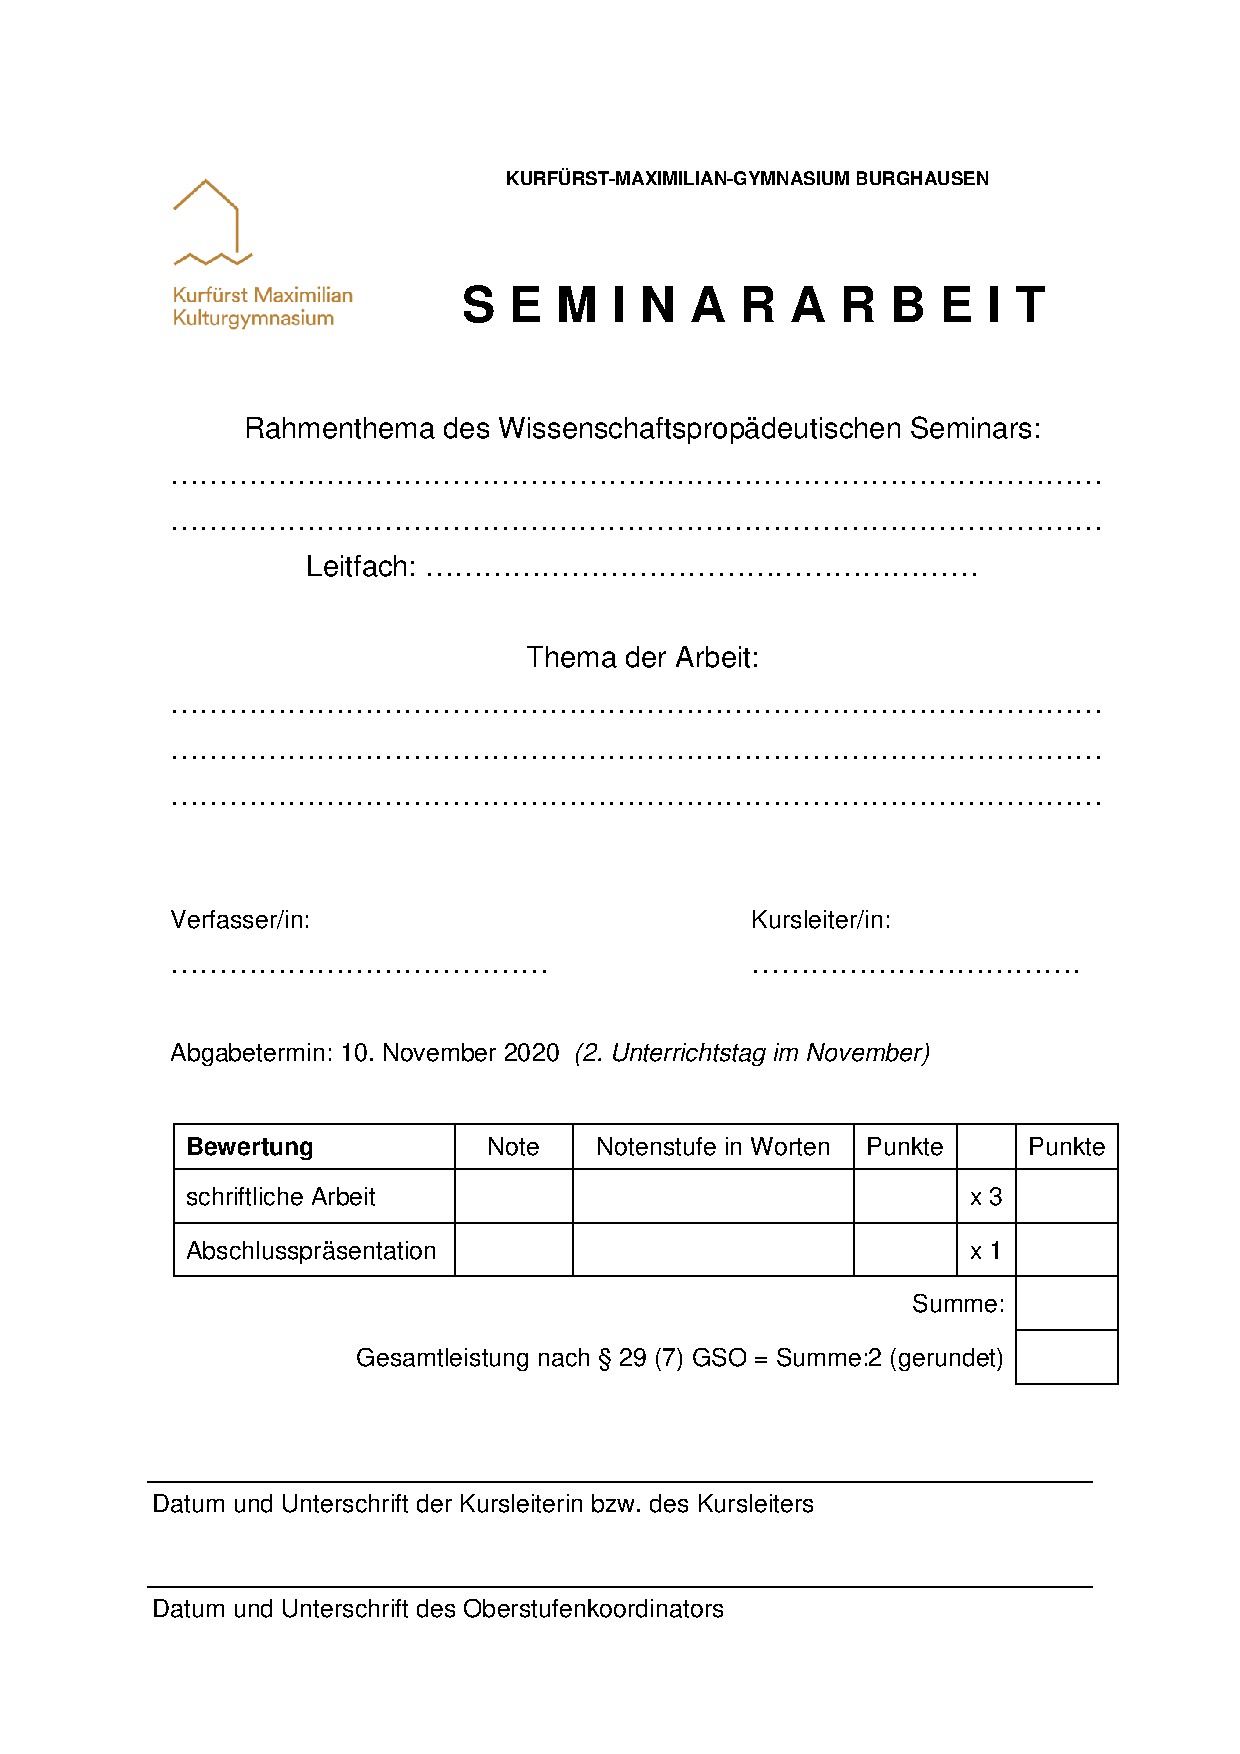
\includepdf[pages=-]{./content/Deckblatt_Seminararbeit_2020.pdf}
    \maketitle
    \newpage
    \tableofcontents
    \newpage
    \pagenumbering{arabic}

    \section{Einleitung}
    Bei der Betrachtung der Benennung der Epochen in der menschlichen Geschichte ist bemerkbar, dass hier mehrmals die bedeutendste technische Errungenschaft aus diesem Zeitraum zur Namensgebung verwendet wird. Das ist natürlich sinnvoll da diese Entwicklungen im großen Ausmaß das Leben der Menschen beeinflussten und auch für den weiteren Verlauf der Geschichte ausschlaggebend sind. Diese Namen sind  wie \enquote{Bronzezeit} recht selbsterklärend, hier wurde die Metallverarbeitung, vor allem mit Bronze erfunden und revolutionierte die Waffentechnik und ermöglichte auch viele andere neuartige Gegenstände.\footcite{BronzezeitEuropaDeutschland} 
    Schwieriger wird es dann schon bei dem Titel des aktuellen Zeitabschnittes: \enquote{Digitales Informationszeitalter}. Nach \Citeauthor{jornlengsfeld} sind hierbei die \enquote{Informations- und Kommunikationstechnologien} die prägenden Technologien.\footcite{jornlengsfeld}
    Diese Technik hat deshalb eine so große Bedeutung in unserem Leben, da sie uns durch das nicht mehr wegzudenkende Internet jederzeit Zugriff auf eine unfassbare Menge an Informationen verschafft. Allerdings werden auch diese Erfindungen leider nicht immer fortschrittsbringend eingesetzt, sondern sie haben genau wie die Erfindungen des Atomzeitalters ihre Schattenseiten, welche meist zwar um einiges unauffälliger sind, aber nicht immer auch ungefährlicher. Denn gerade diese riesige Reichweite macht das Internet so attraktiv für Angreifer und deshalb mussten Verfahren entwickelt werden um sich gegen Verbrecher, die im Hintergrund mitlesen oder schädliche Informationen verbreiten zu schützen. Aus diesem Grund wurden Verschlüsselungsverfahren entwickelt. Bei \enquote{Verschlüsselung} denkt man zwar schnell an Geheimnachrichten und \enquote*{top-secret} Dokumente, allerdings begegnen wir digitalen Verschlüsselungen inzwischen tagtäglich.

    \section[Verschlüsselung allgemein]{Verschlüsselung im Allgemeinen}
    \subsection{Definition}
    Bei der Verschlüsselung handelt es sich um eine Form der Codierung, hierzu gehört zum Beispiel auch der \emph{Morsecode} oder die allgegenwärtigen \emph{Borcodes}, allerdings liegt die Zielsetzung bei der Verschlüsselung nicht nur einfach darin die Information in ein anderes Format zu übertragen, sondern hier will man \enquote{die Informationen systematisch so verfälschen, dass sie nicht rekonstruiert werden können, es sei denn, durch ausdrücklich hierzu Berechtigte.} \footcite[263]{dankmeier2006}
    Die Verschlüsselung gehört zum Bereich der \emph{Kryptographie}, womit die \enquote{Wissenschaft vom geheimen Schreiben} \footcite[1]{watjen2008} gemeint ist.

    \subsubsection{Terminologie}
    Aus diesem Wissenschaftsbereich stammen noch mehrere Begriffe ab, die im folgenden von Bedeutung sein werden:
    % Begriffsklärungen %TODO Algorithmus? %TODO Buchstabenabkürzungen hinzufügen
    \begin{description}
        \item[Chiffre] Geheime Methode des Schreibens, also eine Form des Verschlüsselns
        \item[Klartext] Der unverschlüsselte Text
        \item[Chiffretext] Der verschlüsselte Text, bzw. Ausgangstext
        \item[Chiffrieren] Das verschlüsseln des \emph{Klartextes} zum \emph{Chiffretext}
        \item[Dechiffrieren] Das entschlüsseln des \emph{Chiffretextes} um wieder den \emph{Klartext} zu erhalten
    \end{description}

    \subsection[Ziele]{Ziele der Kryptographie}
    % TODO  Nach Moderne Verfahren der Kryptographie (natürlich mit citetitle o.ä)
    % IDEA PIN-Persönliche Identifikationsnummer
    \subsubsection{Geheimhaltung}
    Der wohl bekannteste und offensichtlichste Verwendungszweck der Verschlüsselung ist eine Nachricht geheim zu halten. Hierbei wird die zu übertragende Nachricht so entstellt, dass sie für jeden völlig unsinnig erscheint, außer für den beabsichtigten Empfänger, welcher den geeigneten Schlüssel besitzt, er ihm das Dechiffrieren ermöglicht.\footcite{beutelspacher2015}
    \subsubsection{Authentikation}
    Bei der Authentikation liegt das Ziel darin, die Echtheit einer Identität oder Nachricht zu überprüfen, da wir uns in der digitalen Welt nicht einfach durch unser Aussehen oder unsere Stimme ausweisen können und auch bei Nachrichten ist nicht zweifelsfrei Festzustellen von wem sie versendet hat und ob sie auf ihrem Weg verändert wurden. Zur \emph{Teilnehmerauthentikation} gehört unter anderem das eingeben der Geheimzahl am Geldautomaten, da nur der Besitzer der EC-Karte auch die dazu gehörige Nummer kennt und so seine Identität dem Geldautomaten nachweisen kann. Hier gilt das Prinzip:
    \begin{quote}
        Ich weise meine Identität dadurch nach, dass ich nachweise, etwas zu haben, was kein anderer hat.\footcite{beutelspacher2015}
    \end{quote}
    Ähnlich funktioniert es bei der \emph{Nachrichtenauthentikation}: hier verknüpft der Ersteller sein \enquote{Geheimnis} mit dem Dokument um es authentisch zu machen. Im Falle des Bankautomaten, muss allerdings zusätzlich zum Kontoinhaber logischerweise auch der Bankautomat die Geheimnummer kennen. Es gibt aber auch sogenannte \emph{Signaturverfahren}, bei denen dies nicht notwendig ist.
    \subsubsection{weitere Ziele}
    Neben den beiden oben genannten Zielen für die die RSA-Verschlüsselung am häufigsten eingesetzt wird, gibt es auch noch weitere Ziele, die zwar weniger prominent sind, jedoch ähnliche Techniken nutzen. Bei dem Zeil der \emph{Anonymität} wird die Identität verborgen, was bei einer digitalen Geschäftsabwicklung mit dem Zahlen mit Bargeld verglichen werden kann, aber auch oft zum Schutz der Privatsphäre eingesetzt wird. Wie die RSA-Verschlüsselung basieren \emph{kryptographische Protokolle} größtenteils auf dem \emph{Public-Key-Verfahren}. Mit einem Protokoll wird hierbei die zum Datenaustausch nötige Abfolge von auszuführenden Schritten bezeichnet. Somit ist es durch vorher festgelegte Protokolle möglich, dass sich eine große Anzahl von Teilnehmern miteinander verschlüsselt verständigen können. Ein \emph{kryptografisches Protokoll} muss sich aber nicht auf den digitalen Nachrichtenaustausch beschränken, sondern auch schon das Bedienen eines Bankautomaten wird als solches bezeichnet.

    \subsection{Klassische Chiffren} % FIXME bessere Überschrift
    Die Verschlüsselung kann auf eine lange Entwicklungsgeschichte zurückblicken, und laut \textcite[28]{ertel2003} werden alle Verfahren, die bis etwa 1950 entwickelt und verwendet wurden als \emph{klassische Chiffren} bezeichnet. Diese Chiffren können in \emph{Transpositionschiffre} und \emph{Substitutionschiffre} unterteilt werden.    % FIXME mehr Zitationen?
     Bei einer \emph{Transpositionschiffre} wird die Anordnung der Zeichen im Chiffretext gegenüber dem Klartext verändert, die Zeichen an sich aber bleiben dabei gleich. Im Chiffretext einer \emph{Substitutionschiffre} dagegen bleibt die Position des Zeichens erhalten, jedoch wird das Zeichen an sich ersetzt. Diese lässt sich noch weiter \emph{monoalphabetische}, bei der ein Klartext-Zeichen im Chiffretext immer durch das gleiche Zeichen repräsentiert wird und \emph{polyalphabetische}, bei der sich das zugehörige Chiffretext-Zeichen abhängig vom Kontext verändert.
    \subsubsection{Caesar-Verschlüsselung}
    Die nach ihrem berühmtesten Benutzer \person{Julius Caesar} benannte Chiffre ist zwar keine besonders sichere, aber zur Veranschaulichung gut geeignet. Diese Chiffre ist eine \emph{monoalphabetische Substitutionschiffre} und kann noch genauer den \emph{Verschiebechiffren} zugeordnet werden. Wie es durch den Namen bereits suggeriert wird, wird der Klartext durch Verschiebung seiner Zeichen chiffriert. Bei der Caesar-Verschlüsselung wird dies erreicht, indem jedes Zeichen mit dem Zeichen ersetzt wird, das an der Stelle im verwendeten Alphabet steht, die sich aus der Position des Klartext-Zeichens im Alphabet, summiert mit dem Schlüssel ergibt. Allgemein kann dies mit folgender Formel beschrieben werden:
    \begin{equation}
        z \mapsto (z+k) \bmod n
    \end{equation}
    Hierbei steht $z$ für das Klartextzeichen und $k$ für den Schlüssel. Zusätzlich wird durch das Modulo verhindert, dass des Chiffre-Zeichen außerhalb des Alphabets liegt, wobei $n$ die Länge des Alphabets angibt. Bei $k=3$, wie \person{Julius} es verwendete, ergibt sich dann folgende Klartext-Alphabet zu Chiffre-Alphabet Zuordnung:
    \begin{center}
        \begin{tabularx}{\textwidth}{r*{26}{C}}
            Klartext: &a&b&c&d&e&f&g&h&i&j&k&l&m&n&o&p&q&r&s&t&u&v&w&x&y&z\\
            Chiffretext: &D&E&F&G&H&I&J&K&L&M&N&O&P&Q&R&S&T&U&V&W&X&Y&Z&A&B&C       
        \end{tabularx}
    \end{center}
    Wenn dieses Vorgehen jetzt auf einen Text angewendet wird, entstehen Ergebnisse, die in etwa so aussehen:
    \begin{center}
        \begin{tabular}{ccc}
            seminararbeit & hallo welt & schule \\
            $\downarrow$ & 	$\downarrow$ & 	$\downarrow$\\
            VHPLQDUDUEHLW & KDOOR ZHOW & VFKXOH
        \end{tabular}
    \end{center}
    Die Entschlüsselung erfolgt hier mit dem selben Schlüssel, der auch bei der Verschlüsselung verwendet wurde, indem die Buchstaben in entgegengesetzte Richtung verschoben werden. Diese Art der Verschlüsselung ist allerdings sehr unsicher, da sie mehrere Problemstellen aufweist:
    \begin{description}
        \item[Die Schlüsselübertragung] Verschlüsselung wird häufig benutzt, wenn damit gerechnet wird, dass die Kommunikation abgehört wird. Da aber um die verschlüsselte Kommunikation herzustellen zuerst der Schlüssel ausgetauscht werden muss, stellt sich hier die Frage, wie das erreicht werden kann, ohne dass der ungewollte Dritte davon Kenntnis nimmt.
        \item[Schlüsselmöglichkeiten] Es gibt hier nur eine sehr begrenzte Anzahl von Zahlen, die für $k$ eingesetzt werden können, und zwar $n-1$. Theoretisch können auch größere Zahlen eingesetzt werden, allerdings erzeugen sie aufgrund des Modulo keine neuen Chiffretexte. Durch diese begrenzten Variationen ist es möglich den Klartext zu ermitteln, indem alle möglichen Schlüssel durchprobiert werden.
        \item[Monoalphabetisch] Da es sich um eine \emph{monoalphabetische} Verschlüsselung handelt, kann der Schlüssel ermittelt werden, indem die statistische Verteilung der Buchstaben im Chiffretext mit dem durchschnittlichen Auftreten in der jeweiligen Sprache verglichen wird.
    \end{description}

    \subsection{Symmetrie}  %FIXME Ziatation
        Eine weitere wichtige Unterteilung der Verschlüsselungsformen ist die \emph{Symmetrie}. (vgl. \cite{ertel2003}[18]) Hier wird unterschieden, ob die Entschlüsselung mit dem gleichen Schlüssel wie die Verschlüsselung erfolgt, dies wird als \emph{symmetrisch} bezeichnet, oder ob für die Entschlüsselung ein separater Schlüssel verwendet werden muss (\emph{asymmetrisch}). Wenn nun $E$ die Verschlüsselung (encryption), $D$ die Entschlüsselung (decryption), $M$ den Klartext, $C$ den Chiffretext (ciphertext) und $K$ den Schlüssel (key) bezeichnet, gilt für einen \emph{symmetrischen Algorithmus}: %FIXME wenn in Terminologie erwähnt, hier die Buchstaben Raus
        \begin{align}
            E_K(M) &= C\\
            D_K(C) &= M\\
            D_K\left(E_K(M)\right) &= M
        \end{align}
        Für einen \emph{asymmetrischen Algorithmus} gilt nahezu identisches, mit dem Unterschied, dass für die Verschlüsselung der Schlüssel $K_1$ und für die Entschlüsselung $K_2$ verwendet wird:    %FIXME Seitenumbruch
        \begin{align}
            E_{K_1}(M) &= C \label{eq:funf} \\
            D_{K_2}(C) &= M \label{eq:sechs}    \\
            D_{K_2}\left(E_{K_1}(M)\right) &= M     \label{eq:sieben}
        \end{align}
        %TODO Injektivität? Ertel 18

        \section{RSA-Verschlüsselung} %FIXME nicht als eigener Unterpunkt?
        \subsection[Public-Key-Kryptosysteme]{Das Public-Key-Verfahren}
        Die Grundlage der RSA-Verschlüsselung bildet die Idee der \emph{Public-Key-Kryptosysteme}.

        \begin{quote}
            [Diese] wurden 1976 von von \emph{W. Diffie} und \emph{M. Hellman} eingeführt. Jeder Benutzer eines solchen Systems hat einen öffentlichen und einen privaten Schlüssel. Damit besitzt jeder Benutzer \emph{A} eine \emph{öffentliche} Chiffriertransformation $E_A$ und eine \emph{private} Dechiffriertransformation $D_A$.\footcite[67]{watjen2008}
        \end{quote} %FIXME anführungszeichen in Blockzitaten?
        Durch diese Form der \emph{asymmetrischen} Verschlüsselung wird das Problem der Schlüsselübertragung behoben, da der zur Verschlüsselung der Nachricht notwendige Schlüssel öffentlich zugänglich ist, die Nachricht jedoch nur mit dem geheimen privaten Schlüssel wieder lesbar gemacht werden kann. Zusätzlich ermöglicht sie durch das Wegfallen des gegenseitigen Schlüsselaustausches auch die verschlüsselte Kommunikation mit jedem beliebigen Partner, ohne die moderner Nachrichtenaustausch durch \enquote{E-Mails} oder \enquote{Instant-Messenger} undenkbar wären.\footcite[Vgl.][21]{ertel2003} Ähnlich zum \emph{asymmetrischen Algorithmus} gilt hier:

        \begin{align}
            E_{P_A}(M) &= C \\
            D_{S_A}(C) &= M \\
            D_{S_A}\left(E_{P_A}(M)\right) &= M
        \end{align}

        Wobei $P_A$ für den öffentlichen Schlüssel (public key) des Teilnehmers $A$ und $S_A$ für den privaten (secret key) steht.\footcite[Vgl.][21f.]{ertel2003}\\
        Beispielhaft wäre damit der Ablauf einer Nachrichtenübertrag folgender:
        \begin{quote}
            Alice ($A$) möchte an Bob ($B$) eine private Nachricht $M$ schicken. Alice kennt Bobs[\footnote{\enquote{\enquote*{Alice} und \enquote*{Bob} als Kommunikationspartner sind Bestandteil der kryptographischen Fachsprache.} \cite[21]{ertel2003}}] öffentlichen Schlüssel und damit $E_B$. Alice bildet den Chiffretext $C = E_B(M)$ und sendet ihn Bob. Nur Bob kennt die Dechiffriertransformation $D_B$, und nur er kann damit den Text durch
            \begin{equation*}
                D_B(C) = D_B(E_B(M)) = M
            \end{equation*}
            entschlüsseln.\footcite[68]{watjen2008}
        \end{quote}
        \begin{center}
            \begin{tikzpicture}[thick, auto]
    \node (input){$M$};
    \node[state, right=of input](encrypt){$E_B$};
    \node[above=of encrypt]{öffentlich};
    \node[below=of encrypt]{Alice};
    \node[state, accepting, right=3cm of encrypt](decrypt){$D_B$};
    \node[above=of decrypt]{privat};
    \node[below=of decrypt]{Bob};
    \node [right=of decrypt](output){$M$};

    \path[->]
        (encrypt) edge node {$C = E_B(M)$} (decrypt)
        (input) edge (encrypt)
        (decrypt) edge (output);
\end{tikzpicture}
\\ %FIXME Abbildungsverzeichnis?
            \emph{Veranschaulichung des Public-Key-Verfahrens\footcite[67]{watjen2008}}\\            
        \end{center}
        Um die Geheimhaltung zu gewährleisten muss das eingesetzte Verfahren so konzipiert sein, dass von dem öffentlichen Schlüssel $P$ keine Rückschlüsse auf den privaten Schlüssel $S$ gezogen werden können.\footcite[49]{beutelspacher2015} %FIXME Seitenumbruch %IDEA Authentikation schon hier?
    
    \subsection{Entwicklung des RSA-Algorithmus}
        Das bis heute wichtigste Public-Key-Kryptosystem\footcite[Vgl.][26]{pieprzyk2010topics} \enquote{wurde 1978 von \emph{R. \textbf{R}ivest},\\ \emph{A. \textbf{S}hamir} und \emph{L. \textbf{A}dleman} erfunden, als sie zu zeigen versuchten, dass Public-Key-Kryptographie unmöglich sei.}\footcite[77]{beutelspacher2015} Dabei war \emph{Rivest} für die Entwicklung des Algorithmus und \emph{Shamir} für die Überprüfung auf Schwachstellen zuständig, während \emph{Adelman} auf beiden Seiten mitwirkte.\footcite[77]{ertel2003} Sie waren jedoch nicht die ersten, denn \enquote{Ende 1997 [wurde bekannt], dass \emph{Clifford Cocks} von den britischen Government Communications Headquarters (GCHQ) bereits 1975 dieselbe Idee hatte, sie aber strenger Geheimhaltung unterlag.}\footcite[71]{watjen2008}%FIXME Zeilenumbruch
    
    \subsection{Schlüsselerzeugung}
        Um die bei einem \emph{asymmetrischen Verschlüsselungsverfahren} nötigen beiden Schlüssel zu erzeugen müssen zuerst zwei unterschiedliche Primzahlen $p$ und $q$ erzeugt werden.(Vgl. \cite[278]{dankmeier2006}) Aus diesen wird dann das Produkt $n=p\cdot q$, den \emph{Modul}, gebildet. Für die Funktionalität des Verfahrens spielt die größe der verwendeten Primzahlen keine Rolle, allerdings sinkt mit steigender Größe die Gefahr des \enquote{Aufbrechens} durch einen Unbefugten, da die Sicherheit der RSA-Verschlüsselung auf dem \emph{Faktorisierungsproblem} beruht. Dies ist \enquote{das bisher ungelöste Problem der schnellen Zerlegung großer Zahlen in ihre Primfaktoren, die Aufgabe hat eine exponentielle Komplexität.}\footcite[279]{dankmeier2006} Dadurch ist es bei den heute verwendten 100- bis 350-stelligen mit aktuellen Methoden und Rechenleistung nicht möglich aus $n$ die zugrundeliegenden Primzahlen $p$ und $q$ zu berechnen. %TODO möglichkeiten um große Primzahlen zu erstellen im nachfolgenden Kapitel, warum überhaupt Primzahlen?
        Zusätzlich zu $n$ muss auch noch die \emph{Eulersche Phi-Funktion} von $n$ gebildet werden.
        \subsubsection{Eulersche Phi-Funktion}
            Die Eulersche $\Phi$-Funktion $\Phi(n)$ bezeichnet die Menge der zu $n$ \emph{teilerfremden} Zahlen $a$ von $1$ bis $n-1$.\footcite[Vgl.][111]{swoboda2008kryptographie}
            \begin{equation}
                \Phi(n)= |\{a\in \left[ 1, n-1 \right] | \ggt(n, a)=1\}|
            \end{equation}
            \enquote{Da alle Primzahlen $p$ nur durch 1 und sich selbst teilbar sind, sind sie sicher zu den Zahlen 1 bis $p-1$ teilerfremd, daher ist $\Phi(p) = p-1$.}\footcite{steinfeld}
            Da $n$ das Produkt zweier verschiedener Primzahlen und somit teilerfremder natürlicher Zahlen ist, gilt die \emph{Multiplikativität}\footcite[Vgl.][]{steinfeld}:
            \begin{equation}
                \Phi(n) = \Phi(pq) = \Phi(p)\cdot\Phi(q)
            \end{equation}
            Für $\Phi(p) = p-1$ und $\Phi(q) = q-1$ ergibt sich also\footcite[Vgl.][279]{dankmeier2006}:
            \begin{equation}
                \Phi(n) = (p-1)\cdot(q-1)
            \end{equation}
        \subsubsection{Das modulare Inverse} %TODO #6 noch ausführlicher (wat40 & dank44)
            \enquote{Des weiteren [wird] eine zu $\Phi(n)$ teilerfremde Zufallszahl $e$ [($1<e<\Phi(n)$)]\footcite[71]{watjen2008} [gewählt] und [...] hierzu die \emph{modulare inverse} Zahl $d$ bezüglich $\Phi(n)$ [berechnet]. Für $d$ gilt:}\footcite[279]{beutelspacher2015}
            \begin{equation}
                d\cdot e\mod{\Phi(n)} = 1
            \end{equation}
            Da $e$ und $\Phi(n)$ teilerfremd sind, gibt es hierfür eine eindeutige Lösung\footcite[Vgl.][77, 164]{ertel2003}. Dieses
            \enquote{$d$ kann berechnet werden mit dem \emph{erweiterten Euklidischen Algorithmus}.}\footcite[77]{ertel2003}

        \paragraph{Der erweiterte Euklidische Algorithmus}
            Lorem ipsum %muss noch was rein, rekursion und so weiter
        % was bringt das überhaupt
        \subsubsection{Die Schlüssel}
            Mit diesen berechneten Zahlen können nun die Schlüssel erstellt werden(Vgl. \cite[77]{ertel2003}):
            \begin{description}
                \item[Der öffentliche Schlüssel ($P$)] besteht aus dem Paar $P=(e, n)$ und wird allen Personen, von denen der Besitzer Informationen erhalten will, zugänglich gemacht. Hier wird auch erkenntlich, weshalb es so wichtig ist, dass $n$ nicht leicht in seine Primfaktoren zerlegt werden kann, denn wenn es einem Angreifer gelingen sollte diese ausfindig zu machen könnte er damit den \emph{privaten Schlüssel} berechnen und alle (abgefangenen) Nachrichten zu entschlüsseln.
                \item[Der geheime Schlüssel ($S$)] wetzt sich aus $S=(d, n)$ zusammen und sollte nur dem Besitzer bekannt sein. 
            \end{description}
            Da die Schlüsselerzeugung meist von einer Schlüsselvergabestelle, wie z.B. dem Anbieter Sofortnachrichtendienstes, sollte dieser nach Berechnung der Schlüssel die Primzahlen $p$ und $q$, sowie das Ergebnis der zugehörigen Eulerfunktion $\Phi(n)$ löschen, damit auch im Falle einer Kompromittierung der Server dessen die Privatsphäre der Nutzer geschützt ist.\footcite[279]{dankmeier2006} %CHECK Grammatik "Server dessen" oder Bezug auf Vergabestelle? %TODO Ablaufschema: Cryptool oder tikz

    \subsection{Ver- und Entschlüsselungs Algorithmus}
            Möchte Bob nun eine chiffrierte Nachricht an Alice verschicken, muss er folgendermaßen vorgehen (Vgl. \cite[71]{watjen2008}):
            \begin{enumerate}
                \item Bob beschafft sich den öffentlichen Schlüssel $P$ von Alice
                \item Da die Buchstaben seiner Nachricht nicht direkt verschlüsselt werden, muss er sie in Zahlen übersetzen, die in $\mathbb{Z}_n$ enthalten sein müssen. %CHECK was ist Zn
                \item
                Mit der Chiffrierfunktion \ref{eq:encryption}\footcite[77]{ertel2003} verschlüsselt Bob alle Buchstaben und übermittelt den ermittelten Geheimtext an Alice.
                \begin{equation}
                    E(M) = M^{e}\mod{n} \label{eq:encryption}
                \end{equation}
            \end{enumerate}
            In Abbildung \ref{fig:encrypt} wurde der Ablauf einer Verschlüsselung mit dem Programm \textbf{Cryptool 2} veranschaulicht. Aus Gründen der Übersichtlichkeit wurde hier anstelle der einzelnen Buchstaben der gesamte Text in eine Zahl umgewandelt und die Schlüsselgenerierung wurde dem Programm überlassen.
            % TODO Programm richtig zitieren
            \begin{figure}
                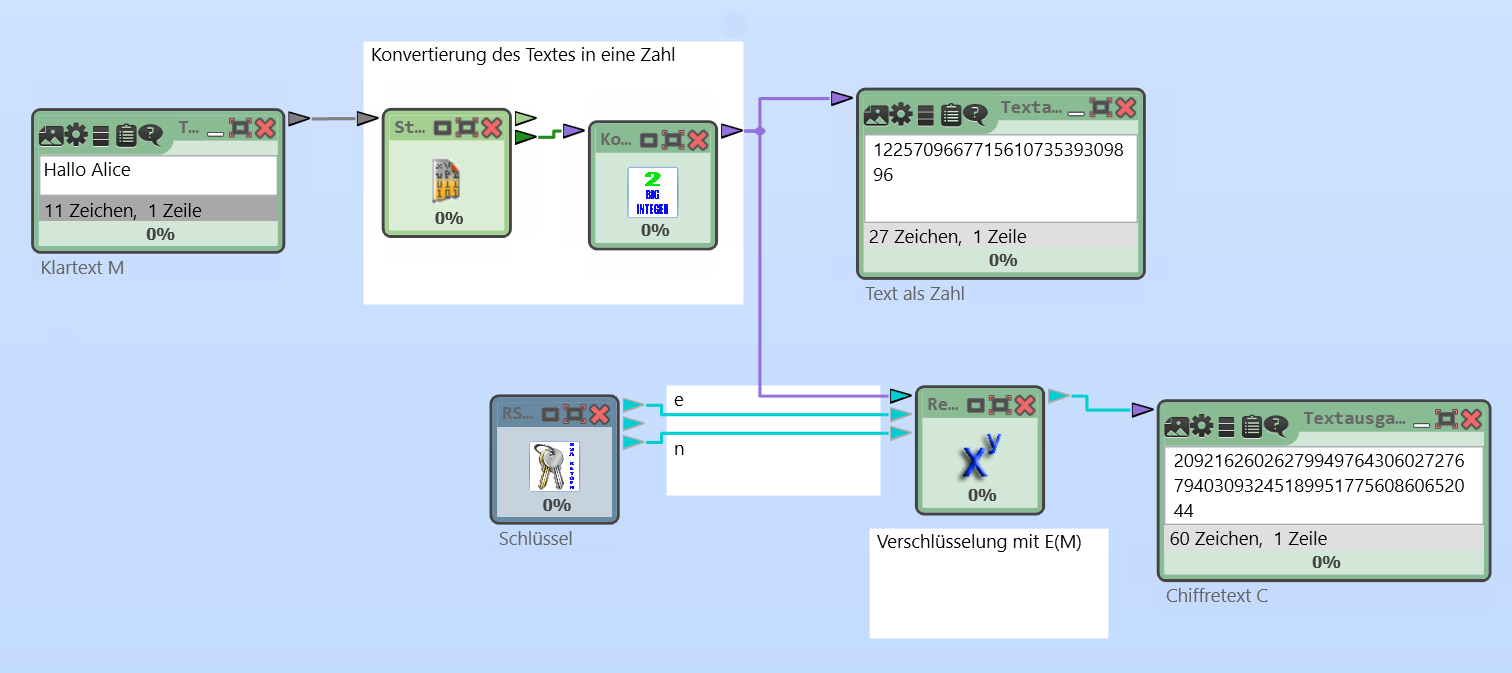
\includegraphics[width=\linewidth]{content/cryptool_encrypt_e1.png}
                \caption{Veranschaulichung des Verschlüsselungprozesses}
                \label{fig:encrypt}
            \end{figure}
            % TODO Abbildungsverzeichnis

            Um Bobs Nachricht lesen zu können, muss sie den Chiffretext mit der Dechiffrierfunktion \ref{eq:decrytion} entschlüsseln und wieder zurück in Buchstaben konvertieren.\footcite[77]{ertel2003}
            \begin{equation}
                D(C) = C^{d}\mod{n} \label{eq:decrytion}
            \end{equation}
            \begin{figure}
                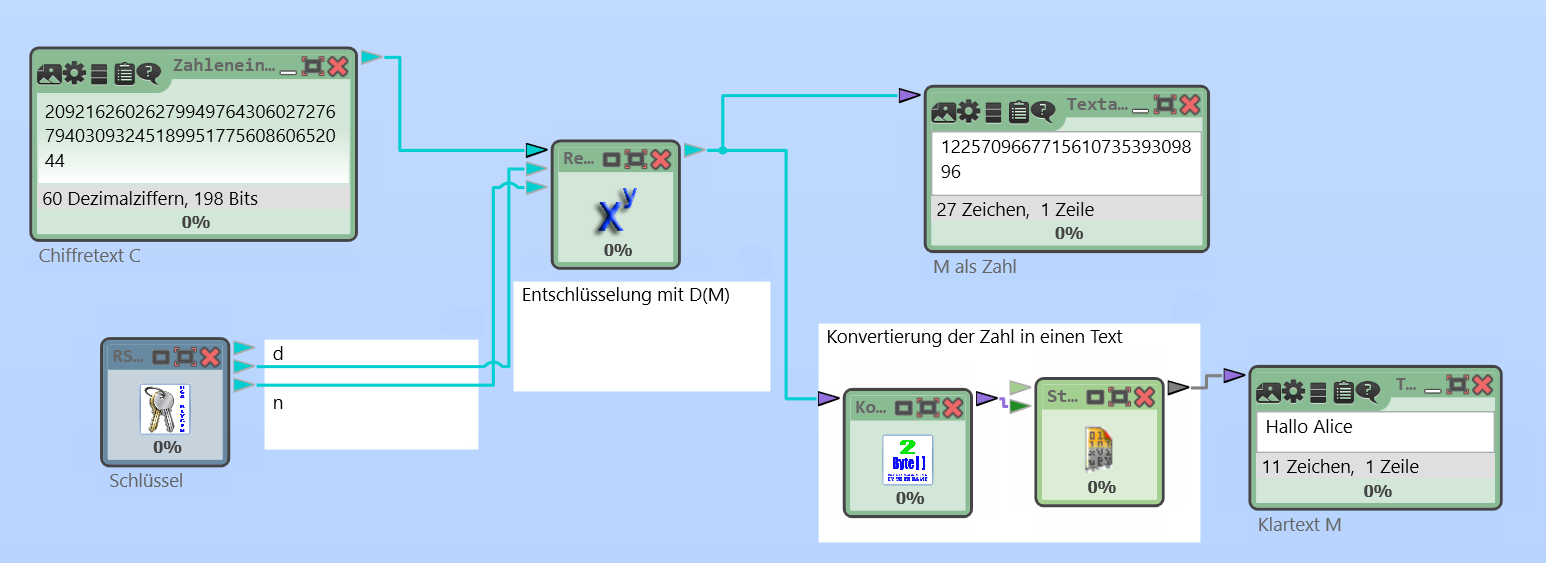
\includegraphics[width=\linewidth]{content/cryptool_decrypt_e1.png}
                \caption{Veranschaulichung des Entschlüsselungprozesses}
                \label{fig:decrypt}
            \end{figure}
            %TODO noch was dazu schreiben?
            %TODO Bilder noch besser anordnen?

    %TODO Beispiel
    %TODO Algorithmus in Terminologie einbinden

    \subsection{Signatur}

    \subsection{Beweis}

    \subsection{praktische Anwendungen}

    \subsection{Vor-  Nachteile}

    \section{Schluss/Ausblick}

    \newpage
    \printbibliography
    \newpage
    \section*{Erklärung}

\vspace{0.2cm}

Ich versichere, dass ich die Seminararbeit ohne fremde Hilfe angefertigt und nur die im Literaturverzeichnis angeführten Quellen und Hilfsmittel benützt habe.

\vspace{1.8cm}

\noindent   \dotfill   \hspace{2.5cm}  \dotfill

\hspace{1.29cm}   Ort und Datum \hfill Unterschrift \hspace{2.15cm}


\end{document}
